\documentclass{beamer}
% September 2014 
% Author: Dr Rachid Hourizi and Dr. Michael Wright 
% Department of Computer Science, University of Bath
\usepackage{listings}
\usetheme{Boadilla} 
\lstset{language=c,
	basicstyle=\ttfamily\small,
           keywordstyle=\color{blue}\ttfamily,
           stringstyle=\color{red}\ttfamily,
           commentstyle=\color{green}\ttfamily,
          breaklines=true}

\begin{document}

\AtBeginSection[]{
  \begin{frame}
  \vfill
  \centering
  \begin{beamercolorbox}[sep=8pt,center,shadow=true,rounded=true]{title}
    \usebeamerfont{title}\insertsectionhead\par%
  \end{beamercolorbox}
  \vfill
  \end{frame}
}

\title{CM10227/ CM50258: Lecture 5}
\author{Dr Rachid Hourizi and Dr. Michael Wright}
\date{\today}
\frame{\titlepage}

\begin{frame}
\begin{center}
\textbf{Resources}
\end{center}
\begin{itemize}
\item More help with this course
\begin{itemize}
\item Moodle
\item E-mail - programming1@lists.bath.ac.uk
\end{itemize}
\item Online C \alert{and Java} IDE
\begin{itemize}
\item \url{https://www.codechef.com/ide}
\item Remember to select Java from the drop down menu.
\end{itemize}
\item Books
\begin{itemize}
\item C by Dissection
\item Java by Dissection (Free pdf online)
\end{itemize}
\end{itemize}
\end{frame}

\begin{frame} 
\begin{itemize}
\item The places that you can get additional support if you are finding the pace of the course a little fast now include
\begin{itemize}
\item \text{The A labs}
\item \text{The B (catch up) lab}
\item \text{The Drop in Sessions}
\end{itemize}
\item please note that we have moved a couple of the labs
\item please check the details on Moodle and let us know if you now cannot get to a lab that you wold otherwise have attended.
\end{itemize}
\end{frame}

\begin{frame}
\begin{itemize}
\item If you struggling with the exercises, pace of the course and/or coding in general
\item Please come and see Rachid or Michael
\end{itemize}
\end{frame}
 
\begin{frame} 
\begin{itemize}
\item If, on the other hand, you are finding the pace a little slow  
\item You can still sign up for the Advanced Programming Labs
\end{itemize}
\end{frame}

\begin{frame}
\begin{center}
\textbf{Last Week}
\end{center}
\begin{itemize}
\item Complex Collections (In C)
\item Abstract Data Types (In C)
\end{itemize}
\end{frame}

\begin{frame}
\begin{center}
\textbf{This Week}
\end{center}
\begin{itemize}
\item Java
\item First Java Program
\item Objects
\end{itemize}
\end{frame}

\section{Java}
\begin{frame}{}
\begin{itemize}
\item This week marks a major turning point in the course
\begin{itemize}
\item We will move from using C
\item To using a second programing language: Java
\end{itemize}
\item (We will talk more about why later in the lecture)
\end{itemize}\end{frame}\begin{frame}\begin{itemize}

\item That change means that you will have to learn
\begin{itemize}
\item new ways to write the instructions that we want the computer to execute and
\item a new way to think about the programs that we write whilst using
those instructions: Object Oriented Programming
\end{itemize}
\end{itemize}\end{frame}

\begin{frame}\begin{itemize}

\item As you make these changes, however, it is worth noting that you are
not starting from scratch

\begin{itemize}
\item When writing small Java programs, the programs that you write can appear reasonably
similar to those that you wrote in C
\item The Java version of HelloWorld, for example, bears some similarity
to the C version

\end{itemize}
\end{itemize}\end{frame}

\begin{frame}[fragile]
\begin{block}{}
\begin{lstlisting}
public class HelloWorld {

    public static void main(String[] args) {
        
	//print HelloWorld to the terminal
        System.out.println("Hello, World");
    }

}
\end{lstlisting}
\end{block}
\end{frame}

\begin{frame}
\begin{itemize}
\item Similarities with the C version of HelloWorld include
\begin{itemize}
\item The presence of a main method (starting point for the flow of execution) - Vocabulary note: method not function in this case
\item A pre-defined instruction to print ``Hello World'' to the screen
\item Some kind of input to the main method (String[] args)
\item A familiar return type (void)
\item the use of a semicolon (;) to mark the end of an instruction
\end{itemize}
\end{itemize}
\end{frame}

\begin{frame}
\begin{itemize}
\item Differences from the C version of HelloWorld include
\begin{itemize}
\item The keyword class
\item The keyword public (formally, an ``Access modifier'' - we will return to this later)
\item The keyword static (again, an element to which we will return later)
\item Slightly different syntax for comments - //
\item Different syntax for the print command - System.out.println() 
\end{itemize}
We will return to each of these differences later
\end{itemize}
\end{frame}

\begin{frame}\begin{itemize}

\item To some extent, you will also see similarities between 

\begin{itemize}
\item the ways in which you compile and run a Java program and
\item the ways in which you compile and run a C program
\end{itemize}
\item These similarities can be misleading, however

\begin{itemize}
\item On closer examination, the steps taken to prepare a Java program for
execution
\item Are different from those taken when preparing a C program
\end{itemize}
\end{itemize}\end{frame}

\begin{frame}
\begin{itemize}
\item Java programs are both compiled and
interpreted.  
\item Instead of translating Java programs into a 
machine language, the Java compiler generates Java byte code for its \alert{Virtual Machine}
\begin{itemize}
\item Byte code is easy (and fast) to interpret, like machine language,
\item but it is also portable, like a high-level language.  
\end{itemize}
\item Thus, it is possible to compile a Java program on one machine,
transfer the byte code to another machine over a network,
and then interpret the byte code on the other machine.  
\item This ability is one of the advantages of Java over many other
high-level languages.
\end{itemize}
\end{frame}

\begin{frame}[fragile]
\begin{itemize}
\item We can use compilation/interpetation of the HelloWorld program on an earlier slide as an example:
\item Before you start, the filename in which you save your main method should match the name of the class with the extension .java. In this case, HelloWorld.java
\item Note: Java is \alert{case sensitive}, just like C.
\end{itemize}
\end{frame}

\begin{frame}[fragile]
\begin{itemize}
\item To run the code:
\item we need to compile it: \lstinline!javac HelloPrinter.java!
\item This will generate a file \lstinline!HelloPrinter.class!, containing the virtual machine byte code
\item We can now run the code by typing the name of the class file
\item NB When running a Java file, you omit the .class suffix:
\end{itemize}
\begin{block}{}
\begin{lstlisting}
$javac HelloWorld.java
$java HelloWorld
Hello, World
\end{lstlisting}
\end{block}

\end{frame}

\begin{frame}[fragile]
\begin{itemize}
\item If you write a program involving multiple classes,
\item you would normally save each  class in a different file
\item Note: Each file must have a name of the form [classname].java
\item where [classname] is the name of the class contained in the file
\end{itemize}
\end{frame}

\begin{frame}[fragile]
\frametitle{A Shortcut:}
\begin{itemize}
\item If you have multiple java files, you can compile tham all with one command. 
\item i.e. You can use \lstinline!javac *.java! to compile all .java files in the current directory in one go.
\item To run the program, you then need to use the interpreter command (\lstinline!java!) on the class that contains the \lstinline!main! method. 
\item We will discuss multi-class programs shortly
\begin{block}{}
\begin{lstlisting}
$javac *.java
$java HelloWorld
Hello, World
\end{lstlisting}
\end{block}
\end{itemize}
\end{frame}

\begin{frame}\begin{itemize}

\item Just as you did with C,

\item We would strongly suggest that you adopt an iterative approach to
developping Java programs i.e.

\begin{itemize}
\item start with a program that works 
\item (such as the Java version of HelloWorld introduced earlier)
\item and extend/debug it in small increments
\item until you have a program that does what you want
\end{itemize}
\end{itemize}\end{frame}


\begin{frame}
\begin{itemize}
\item In order to go beyond our HelloWorld program, however
\begin{itemize}
\item You will need to understand that Java is an Object Oriented (OO) language
\item (Sometimes described as an Object Oriented Programming (OOP) language)
\end{itemize}
\end{itemize}
\end{frame}

\begin{frame}\begin{itemize}
\item This begs two obvious questions:
\begin{itemize}
\item What does it mean to be ``Object Oriented'' when
writing code?
\item And, in a programming context, what is an
Object anyway?
\end{itemize}
\end{itemize}
\end{frame}

\begin{frame}
\begin{itemize}
\item Object Oriented Programming: A type of programming in which programmers
define not only the data type of a data structure, but also the types
of operations (methods) that can be applied to the data structure.
In this way, the data structure becomes an object that includes both
data and functions.
\tiny
\item http://www.webopedia.com/TERM/O/object\_oriented\_programming\_OOP.html
\end{itemize}
\end{frame}


\begin{frame}
\begin{itemize}
\item In other words, an Object Oriented Programming approach maintains this interest in associating
data with the operations that can be performed on it:
\end{itemize}
\end{frame}

\begin{frame}
\frametitle{How does Java ``support'' an OO approach to programming?}
\begin{itemize}
\item C allowed us to use 
\begin{itemize}
\item \textbf{data structures} and 
\item \textbf{functions} which allow us to manipulate those structures
\end{itemize}
\item Java forces us to use 

\begin{itemize}
\item \textbf{combinations of data structures and functions} (\alert{Objects})

\begin{itemize}
\item some of which are pre-defined for us
\item and some of which we can define ourselves
\end{itemize}
\end{itemize}
\end{itemize}\end{frame}


\begin{frame}
\begin{itemize}
\item For example, if we write a program which stores information about and allows us to print out a Train Ticket
\begin{itemize}
\item i.e. code that  allows us to store an initial cost for the ticket
\item ... update the cost of that ticket
\item and print out the current cost
\end{itemize}
\end{itemize}
\end{frame}


\begin{frame}
\begin{itemize}
\item Java forces us to 
\begin{itemize}
\item \textbf{define} a combination of data and operations once (a \alert{Class})
\item and then \textbf{create} one or more examples (instances) of that class (\alert{Objects})
\end{itemize}
\end{itemize}
\end{frame}


\begin{frame}\begin{itemize}
\item More specifically, each time we want to use a new combination of data
and operations, Java forces us to 

\begin{itemize}
\item start by defining a Class which combines that data and those operations
\item before creating one or more examples of that class (one or more Objects)
\end{itemize}
\item You can think of this process as 

\begin{itemize}
\item defining a template (the Class)
\item and using it to create one or more Objects using that template
\end{itemize}
\end{itemize}\end{frame}

\begin{frame}[fragile]
\begin{block}{}
\tiny
\begin{lstlisting}
public class Ticket
{
    int cost = 10;
    
    //constructor
    public Ticket()
    {
        System.out.println("New Ticket Created!");
    } 
    //mutator
    public void changePrice(int newPrice)
    {
        cost=newPrice;
    } 
    //accessor
    public int getPrice()
    {
        return cost;
    }
}
\end{lstlisting}
\end{block}
\end{frame}

\begin{frame}[fragile]
\begin{block}{}
\begin{lstlisting}
public class TicketMachine
{
    public static void main(String[] args)
    {
    	\\create new Ticket
        Ticket tm = new Ticket();
        
        \\change the price of that ticket
        tm.changePrice(20);
        
        \\retrieve and print the price of that ticket
        System.out.println("" + tm.getPrice());
    }
}
\end{lstlisting}
\end{block}
\begin{block}{}
\begin{lstlisting}
New Ticket Created!
20
\end{lstlisting}
\end{block}
\end{frame}

\begin{frame}
\frametitle{Exercise}
It is useful at this stage to consider some examples of classes (templates) and objects (concrete examples created using those templates):
\begin{tabular}{ll}
TelephoneNumber & lord-of-the-rings \\
BankAccount & Diary\\
harry-potter-and-the-Philosopher-Stone  & myDiary\\
01225-38-5053 & michaelWright\\
Book & Lecturer\\
rachidHourizi & myAccount\\
\end{tabular}
\end{frame}

\begin{frame}
\frametitle{Attributes and Fields}
\begin{itemize}
\item Note from the Ticket example:
\begin{itemize}
\item Just as C Structures contained values stored in member variables
\item an Object has \alert{attributes}: i.e. \alert{values} stored in \alert{fields}. (The data you encapsulate)
\item the class defines what fields an Object has, but each Object stores its own set of values.
The set of values stored in a single Object is called the \alert{state} of the object.
\end{itemize}
\end{itemize}
\end{frame}

\begin{frame}
\frametitle{State}
\begin{itemize}
\item We could also imagine the definition of a circle class (i.e. a template)
\begin{itemize}
\item Which stores information about the diameter, (x and y) position of the centre, colour and visibility of that circle
\end{itemize}
\item And use it to create two different circles
\end{itemize}
\begin{center}
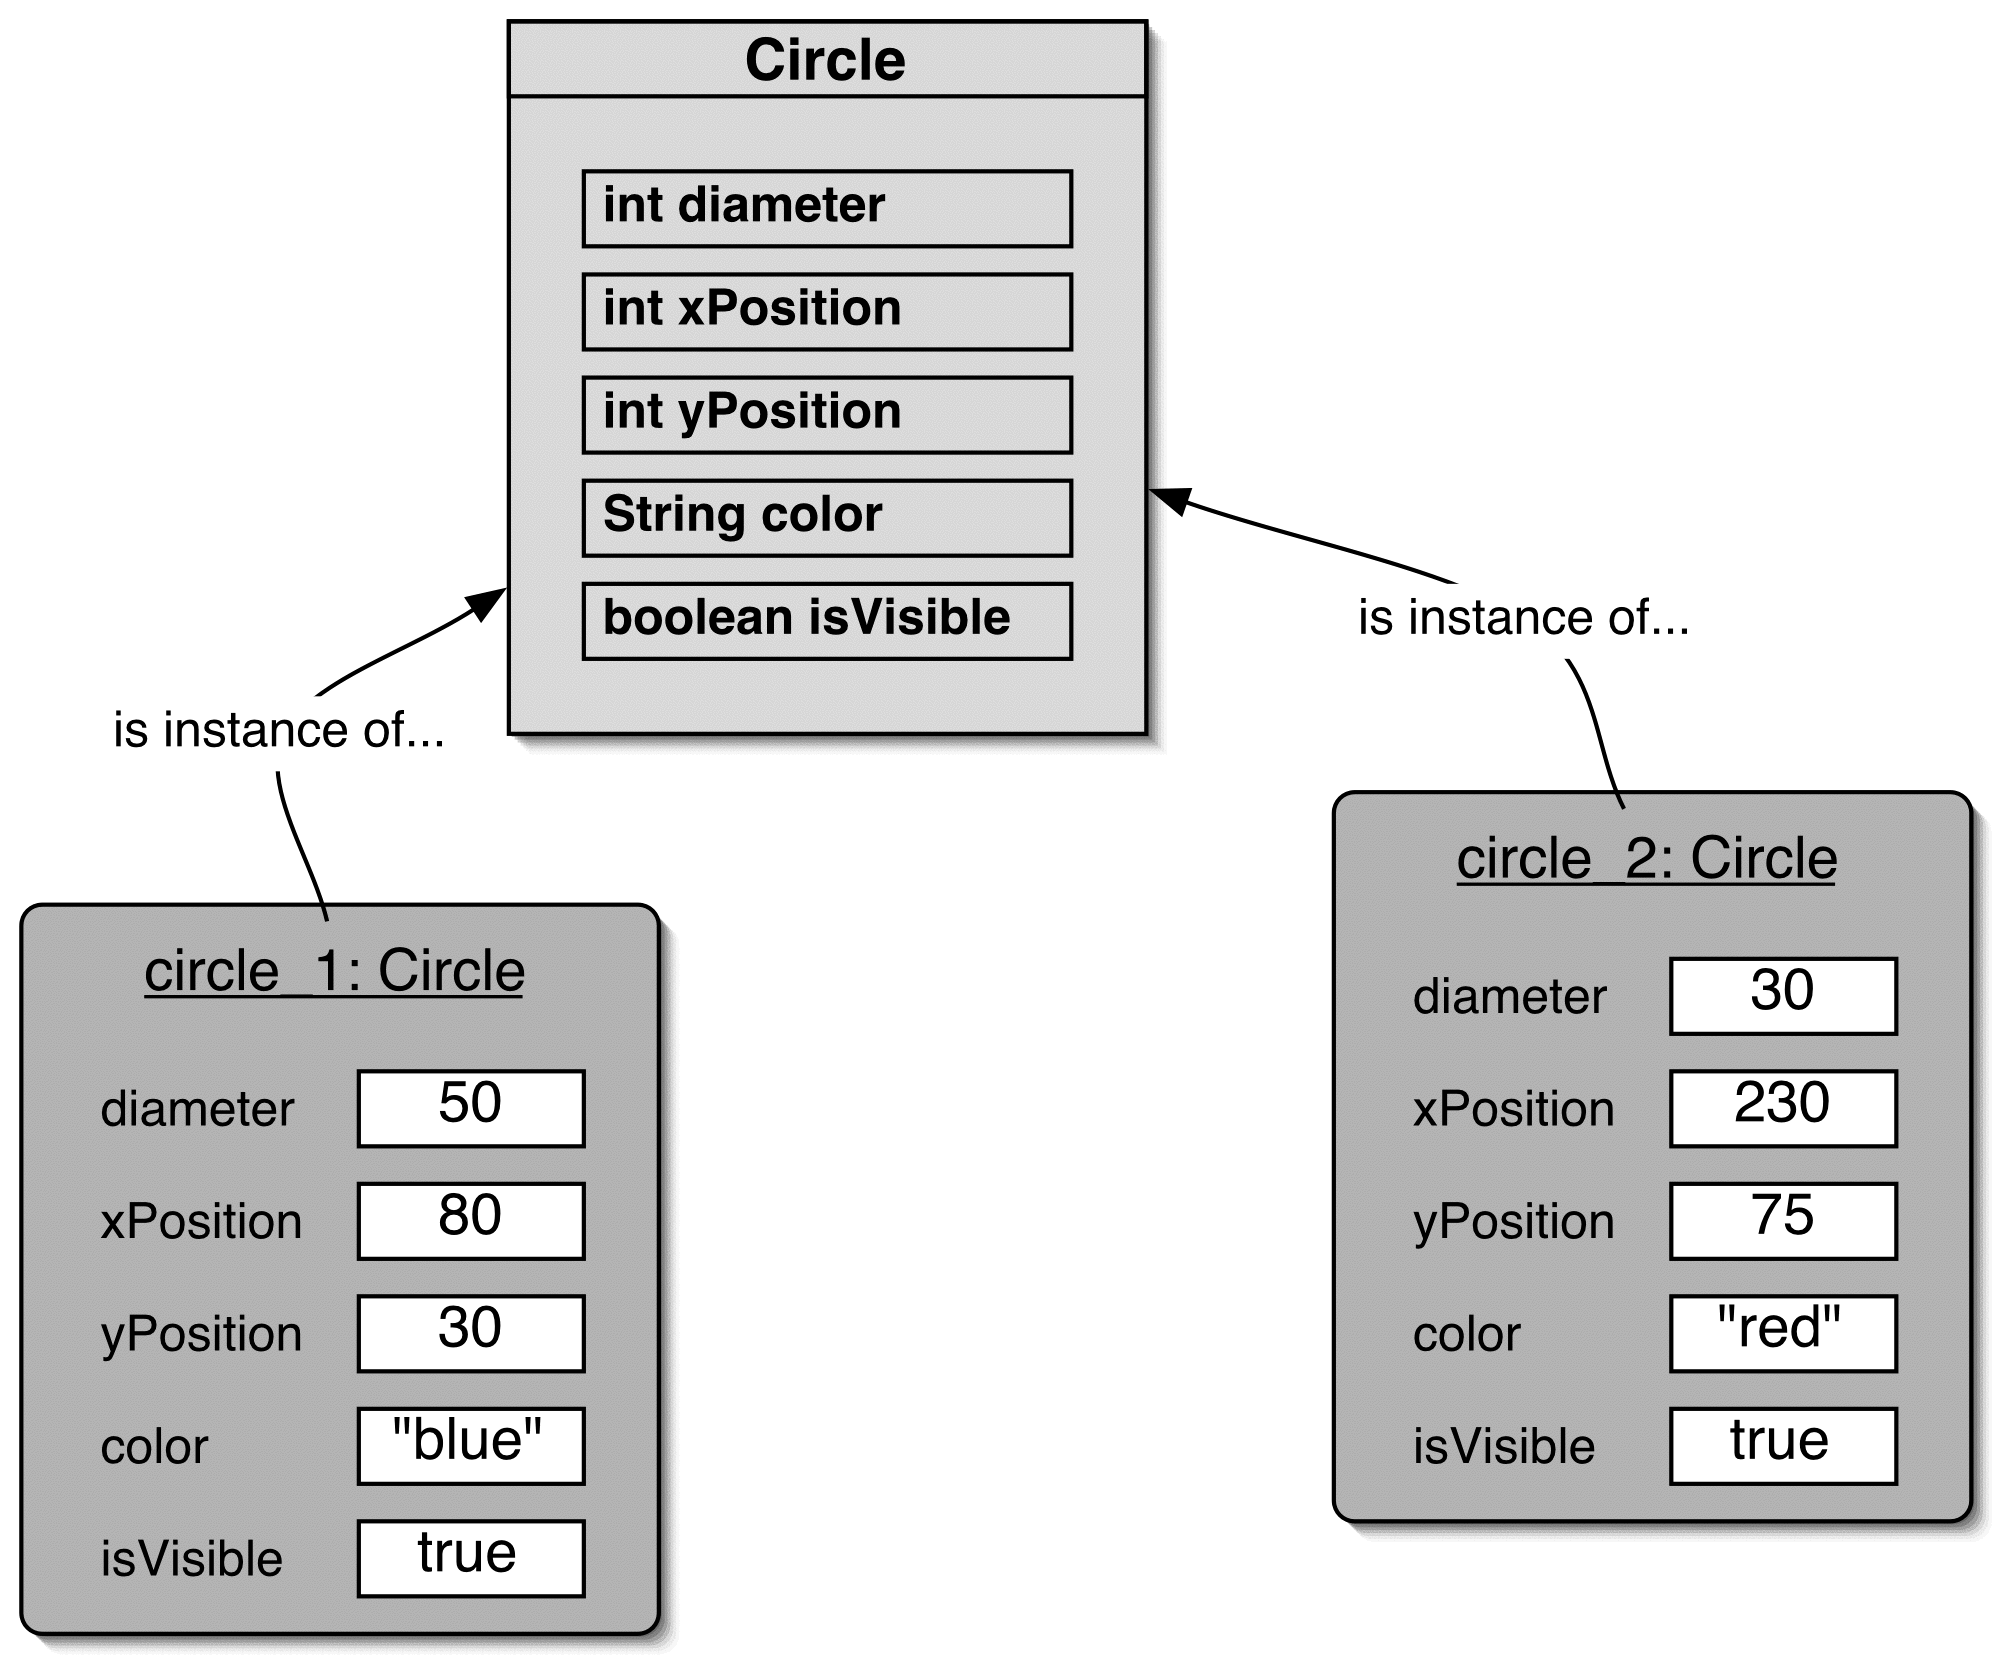
\includegraphics[height=5cm,keepaspectratio]{./figures/state}
\end{center}
\end{frame}


\begin{frame}[fragile]
\frametitle{Methods and Parameters}
\begin{itemize}
\item We also saw previously that objects/classes also have operations which can be invoked. They are called \alert{methods}
\item If, with our Circle example, we wanted to be able to
\begin{itemize}
\item draw examples of the circle class (Circle Objects) on screen and then
\item move those circles a specified distance to the right
\end{itemize}
\item we could include
\begin{itemize}
\item a drawCircle() method in our definition of the Circle class and
\item a moveRight() method in our definition of the Circle class
\end{itemize}
\end{itemize}
\begin{block}{}
\begin{lstlisting}
void moveRight(int distance){
	...some code...
}
\end{lstlisting}
\end{block}
\end{frame}

\begin{frame}
\begin{itemize}
\item The first piece of code used to implement a method e.g.  
\begin{itemize}
\item void moveRight(int distance)
\end{itemize}
\item provides a short description of what the method does
\item that short description is called the method's \alert{signature}
\item The collection of methods in a class is referred to as the \alert{interface} of that class
\end{itemize}
\end{frame}

\begin{frame}
\begin{itemize}
\item Methods are \alert{called} or \alert{invoked}
\item At the point of being called, they may need to recieve information as input if they are to perform the desired operation
\begin{itemize}
\item for example, our moveRight() method may need to be given a distance in order to move a Circle Object as intended
\end{itemize}
\item As in C, that information can be passed in the form of one or more \alert{parameters}
\item in the moveRight(int distance) example, int distance is an example a parameter
\end{itemize}
\end{frame}

\begin{frame}
\frametitle{Data Types}
\begin{itemize}
\item Both Fields and Parameters have \alert{types}. A type defines what kinds of values a parameter can take.
\item In Java (as in C) you have to specify the type.
\item e.g. we know that void moveRight(int distance) takes an integer as input because the distance parameter is defined as being of type int. 
\end{itemize}
\end{frame}

\begin{frame}
\begin{itemize}
\item In Java, everything has a type.
\item Examples of types: int, String, Circle, \ldots
\item Java is \alert{staticly typed language}
\item i.e. once you have given a field or parameter a type, that type cannot change
\item Note: Each time you create a new class, you have defined a new type
\end{itemize}
\end{frame}

\begin{frame}
\frametitle{Source Code}
\begin{itemize}
\item Each class has source code associated with it that defines its details (fields and methods).
\item The code defining each class determines the structure and the behavior of each of its instances (i.e. the structure and behaviour of each Object created using the class template).
\item This source code is compiled and interpreted by Java.
\end{itemize}
\end{frame}

\begin{frame}
\frametitle{Return Values}
\begin{itemize}
\item Methods may return a result via a \alert{return value}.
\item Example: \lstinline!String getName()‏!
This method returns a String.
\item Example: \lstinline!void changeName()‏!
\alert{Void} indicates that this method does not return anything
\end{itemize}
\end{frame}

\begin{frame}
\frametitle{Developing Java Programs}
\begin{itemize}
\item To learn to develop Java programs, one needs to learn how to write class definitions, including fields and methods, and how to put these classes together
\item We will look at these issues in more detail during the remainder of this course
\end{itemize}
\end{frame}

\begin{frame}
Looking at our ticket example in more detail ....
\end{frame}

\begin{frame}[fragile]
\begin{block}{}
\tiny
\begin{lstlisting}
public class Ticket
{
    int cost = 10;
    
    //constructor
    public Ticket()
    {
        System.out.println("New Ticket Created!");
    } 
    //mutator
    public void changePrice(int newPrice)
    {
        cost=newPrice;
    } 
    //accessor
    public int getPrice()
    {
        return cost;
    }
}
\end{lstlisting}
\end{block}
\end{frame}

\begin{frame}[fragile]
\begin{block}{}
\begin{lstlisting}
public class TicketMachine
{
    public static void main(String[] args)
    {
    	\\create new Ticket
        Ticket tm = new Ticket();
        
        \\change the price of that ticket
        tm.changePrice(20);
        
        \\retrieve and print the price of that ticket
        System.out.println("" + tm.getPrice());
    }
}
\end{lstlisting}
\end{block}
\begin{block}{}
\begin{lstlisting}
New Ticket Created!
20
\end{lstlisting}
\end{block}
\end{frame}

\begin{frame}[fragile]
\frametitle{Basic class structure}
\begin{lstlisting}
public class TicketMachine
{
    Inner part of 
    the class omitted.
}
\end{lstlisting}
\end{frame}

\begin{frame}[fragile]
\frametitle{Basic class structure}
\begin{lstlisting}
public class ClassName
{
    Fields
    Constructors
    Mutator Methods
    Accessor Methods
} 
\end{lstlisting}
\end{frame}

\begin{frame}[fragile]
\frametitle{Fields}
Recap:
\begin{itemize}
\item \alert{Fields} store values for an object.
\item They are also known as \alert{instance variables}.
\item Fields define the \alert{state} of an object.
\item Fields have an associated \alert{type}.
\end{itemize}

\begin{lstlisting}
public class TicketMachine
{
    private int price;
    private int balance;
    private int total;
 
    Constructor and methods omitted.
} 
\end{lstlisting}
\end{frame}

\begin{frame}[fragile]
\frametitle{Constructors}
\begin{itemize}
\item Constructors create and initialize an object.
\item Then assign the necessary memory to the created object
\item They have the same name as their class.
\item They store initial values into the fields.
\item They often receive external parameter values for this.
\end{itemize}

\begin{lstlisting}
    //constructor
    public Ticket()
    {
        System.out.println("New Ticket Created!");
    } 
\end{lstlisting}
\end{frame}

\begin{frame}[fragile]
\frametitle{Parameters}
\begin{itemize}
\item Parameter names inside a constructor or method are referred to as \alert{Formal Parameters}
\item Parameter values provided from the outside are referred to as \alert{Actual Parameters}.
\item In the constructor \lstinline!TicketMachine(int ticketCost)! 
\item ticketCost is a 
formal parameter. 
\item When the constructor is called, using \lstinline!TicketMachine(500)!, 
\item 500 is an actual parameter.
\end{itemize}
\end{frame}

\begin{frame}
\frametitle{Scope and Lifetime}
\begin{itemize}
\item The \alert{scope} of a variable/parameter defines the section of the code from which it can be accessed.
\item For instance variables (fields) this is the entire class.
\item For parameters, this is the constructor or method that declares it. 
\item Trick: find the enclosing \{\}, this is the scope. 
\item The \alert{lifetime} of a variable/parameter describes how long the variable continues to exist before it is destroyed.
\end{itemize}
\end{frame}

\begin{frame}[fragile]
\frametitle{Assignment}
\begin{itemize}
\item Similar to C:
\item Values are stored into fields (and other variables) via \alert{assignment} statements:
\begin{itemize}
\item \lstinline!variable = expression;!
\item e.g. \lstinline!price = ticketCost;!
\end{itemize}
\item Both sides of the assignment should have the same type, e.g. int, double, String, TicketMachine, ...
\item A variable stores a single value, so (as in C) any previous value is lost after an assignment.
\end{itemize}
\end{frame}


\begin{frame}[fragile]
\frametitle{Accessor Methods I}
\begin{itemize}
\item All methods implement object behaviour.
\item And all methods have a structure consisting of a header and a body.
\item The header defines the \alert{method’s signature} e.g.   
\begin{lstlisting}
   public int getPrice()‏{
	
	... method body ...

   }

 
\end{lstlisting}

\item The body encloses the method’s statements e.g.
\end{itemize}
\begin{lstlisting}
      ... header{

	   return price;

      }
\end{lstlisting}
\end{frame}

\begin{frame}[fragile]
\begin{itemize}
\item We can, however, be more precise about the kind of behaviour implemented by particular methods
\item \alert{Accessors}, for example are methods which provide information about an object.
\item i.e. they allow users, other programs or other parts of your program to gain information about an object's state
\end{itemize}
\begin{lstlisting}
   public int getPrice()‏
   {
       return price;
   } 
\end{lstlisting}
\end{frame}

\begin{frame}
\frametitle{Mutator Methods}
\begin{itemize}
\item \alert{Mutators} have a similar method structure: header and body.
\item Used to \alert{mutate} (i.e., change) an object’s state.
\item Achieved through changing the value of one or more fields.
\begin{itemize}
\item Typically receive parameters.
\item Typically contain assignment statements.
\end{itemize}
\end{itemize}
\end{frame}

\begin{frame}[fragile]
\frametitle{Mutator methods}
\begin{lstlisting}
    //mutator
    public void changePrice(int newPrice)
    {
        cost=newPrice;
    } 
\end{lstlisting}
\end{frame}

\begin{frame}
\frametitle{Comments/Documentation}
\begin{itemize}
\item As with C, Comments make Java source code easier to read for humans. No effect on the functionality.
\item Three sorts:
\begin{itemize}
\item \lstinline!// comment!: single-line comments
\item \lstinline!/* comments */!: multiple-lines – more detail
\item \lstinline!/** */!: similar to previous, but used when documentation software is used.
\end{itemize}
\end{itemize}
\end{frame}

\begin{frame}
\frametitle{Data Types}
\begin{itemize}
\item As we have seen in the code examples above, Java (like C) provides us with common data types 
\item e.g. integers: 
\begin{itemize}
\item int distance =7;
\end{itemize}
\item you won't be surprised to learn that Java also provides us with chars
\begin{itemize}
\item char myChar ='c';
\end{itemize}
\item booleans
\begin{itemize}
\item boolean a = false; 
\end{itemize}
\item and floats
\begin{itemize}
\item flaot f = 4.0; 
\end{itemize}
\end{itemize} 
\end{frame}

\begin{frame}
\frametitle{Data Types}
\begin{itemize}
\item Java also provides us with ways to implement Strings and Arrays
\item We will return to these data types
\item ..but for now be a little careful with them
\item ..Java and C treat them in rather different ways
\end{itemize} 
\end{frame}

\begin{frame}
\begin{itemize}
\item Each time that we define a class, however, we define a new data type
\item Can be used as parameter, field and return types
\item The internal is hidden from the user
\begin{itemize}
\item No direct access to fields (unless special reason)‏
\item Access to state via accessor and mutator methods
\end{itemize}
\item User does not need to know how the class is implemented to use/instantiate it
\item The usage of a class is defined by its methods
\end{itemize}
\end{frame}

\begin{frame}[fragile]
\frametitle{Making choices}
\small
\begin{lstlisting}
if(perform some test) {
    Do the statements here if the test gave a true result
}
else {
    Do the statements here if the test gave a false result
} 
\end{lstlisting}
\end{frame}

\begin{frame}
\frametitle{Coding Convention}
\begin{itemize}
\item If statement
\begin{itemize}
\item Always use \{ , even if there is only one statement
\item In case there is an else statement, start on a new line and use \{
\end{itemize}
\item Indentation
\begin{itemize}
\item Always indent your code, even if your text editor does not do it automatically
\end{itemize}
\item Document your code, the sooner the better. 
\end{itemize}
\end{frame}

\begin{frame}[fragile]
\frametitle{Boolean Tests}
\begin{itemize}
\item{$==$} : equality
\item{$>$} : greater than
\item{$<$} : less than
\item{$<=$} : less or equal than
\item{$>=$} : greater or equal than
\item{$!=$} : not equal
\end{itemize}
\end{frame}

\begin{frame}
\frametitle{Local variables}
\begin{itemize}
\item Fields are one sort of variable.
\begin{itemize}
\item They store values through the life of an object.
\item They are accessible throughout the class.
\item A bit like global variables in C
\end{itemize}
\item Methods can include shorter-lived variables.
\begin{itemize}
\item They exist only as long as the method is being executed.
\item They are only accessible from within the method.
\item Like function variables in C
\end{itemize}
\end{itemize}
\end{frame}

\begin{frame}[fragile]
\frametitle{Local variables}
\begin{lstlisting}
public int refundBalance()‏
{
    int amountToRefund;
    amountToRefund = balance;
    balance = 0;
    return amountToRefund;
} 
\end{lstlisting}
\end{frame}

\begin{frame}
\frametitle{Review}
\begin{itemize}
\item Class bodies contain fields, constructors and methods.
\item Fields store values that determine an object’s state.
\item Constructors initialize objects.
\item Methods implement the behaviour of objects.
\item Mutators (mutator methods) change the state of a object
\item Accessors (accessor methods) provide information about the state of an object 
\end{itemize}
\end{frame}

\begin{frame}
\frametitle{Review}
\begin{itemize}
\item Fields, parameters and local variables are all variables.
\item Fields persist for the lifetime of an object.
\item Parameters are used to receive values into a constructor or method.
\item Local variables are used for short-lived temporary storage. 
\item Objects can make decisions via conditional (if) statements.
\item A true or false test allows one of two alternative courses of actions to be taken.
\end{itemize}
\end{frame}



\end{document}
